\problemname{Mineralų telkiniai}

\illustration{.3}{img/turnbull.jpg}{Eroding mud face exposing new minerals. Photo: Michael D.\ Turnbull, licence: CC BY-SA.}

\noindent
Jūs dirbate nežemiškų telkinių išgryninimo kompanijai, kurioje užsiimate signalų apdorojimu. 
Šiuo metu jūsų kosminis laivas artėja prie asteroido.
Preliminarūs paviršiaus skenavimai rodo, jog asteroide yra $k$~mineralų telkinių, tačiau jų tikslios vietos nėra žinomos.

\medskip

Asteroido paviršių galima įsivaizduoti kaip koordinačių sistemą.
Kiekvieno mineralų telkinio vieta gali būti nusakoma sveikosiomis koordinatėmis taip, kad 
$i$-ojo telkinio koordinatės yra $(x_i, y_i)$, kur
$-b \le x_i \le b$ ir $-b\le y_i \le b$. %constraint:depositcoords
Čia sveikasis skaičius $b$ yra pradinio skenavimo plotis.

Norėdami nustatyti tikslias mineralų telkinių vietas, galite siųsti zondus į asteroido paviršių.
Zondai siunčiami grupėmis.

Tarkime, jūs norite išsiųsti $d$~zondų grupę į paviršiaus koordinates $(s_j,t_j)$ kiekvienam $1\leq j\leq d$.
Kai zondas atvyksta į savo koordinates, 
jis apskaičiuoja Manhatano atstumą iki kiekvieno iš $k$~mineralų telkinių
ir nusiunčia apskaičiuotus atstumus atgal į kosminį laivą.
Visi duomenų paketai laivą pasiekia tuo pačiu metu, todėl neįmanoma nustatyti, kuris zondas kuriuos atstumus atsiuntė.
Taigi zondų grupė apskaičiuoja ir grąžina $k\cdot d$ sveikųjų skaičių, žyminčių atstumus
\[|x_i-s_j| + |y_i - t_j| \qquad\text{visiems } i \in \{1,\ldots,k\} \text{ ir } j \in\{ 1,\ldots,d\}\,.\]

Jūs norite išsiųsti kuo mažiau zondų grupių į paviršių.


\section*{Bendravimas}

Ši užduotis yra interaktyvi.
Bendravimo pradžioje vienoje eilutėje pateikiami trys sveikieji skaičiai $b$, $k$, and $w$:
koordinačių sistemos riba~$b$,
mineralų telkinių skaičius~$k$,
ir skaičius~$w$ -- kiek daugiausiai zondų grupių galite siųsti.

Tuomet galite klausti $w$ užklausų. Kiekviena jų atitinka vieną grupę.
Užklausa sudaroma iš simbolio \texttt{?}, po kurio pateikiami $2d$ sveikųjų skaičių, atskirtų tarpais.
Taigi užklausos formatas toks: ,,\texttt{?} $s_1$ $t_1$ $\cdots$ $s_d$ $t_d$``, kur zondų skaičiui~$d$ turi galioti
$1\leq d\leq 2000$. % constraint:wavesize
Šios reikšmės $(s_i,t_i)$ nurodo $i$-ojo zondo koordinates ir joms turi galioti
$-10^8 \leq s_i \leq 10^8$ bei $-10^8 \leq t_i \leq 10^8$. % constraint:probecoordinates
Atsakymas į užklausą yra viena eilutėje, kurioje pateikta $k \cdot d$ sveikųjų skaičių, išrikiuotų nemažėjimo tvarka -- 
Manhatano atstumai tarp kiekvienos poros mineralų telkinio ir zondo vietos
Iš viso zondų skaičius, sudėjus visas grupes, negali viršyti
$2\cdot 10^4.$ % constraint:totalprobes

Bendravimas baigiamas, kai išspausdinate vieną eilutę, sudarytą iš simbolio \texttt{!}, po kurio pateikti
$k$ taškų \newline $x_1, y_1, x_2, y_2, \ldots x_k, y_k$, atskirtų tarpais.
Tai turi būti paskutinė jūsų programos išvesties eilutė.

Jūsų sprendimas yra laikomas teisingu, jei išspausdinate visų mineralų telkinių vietas. 
Jas galite spausdinti bet kuria tvarka.

\section*{Ribojimai ir vertinimas}

Visada galios
$1\leq b \leq 10^8$, % constraint:b
$1 \leq k \leq 20$, % constraint:k
ir
$2 \le w \le 10^4$. % constraint:w

Jūsų sprendimas bus testuojamas su keliomis testų grupėmis, kurių kiekviena verta tam tikro skaičiaus taškų.
Kiekviena testų grupė sudaryta iš įvairių testų.
Testų grupės taškai skiriami tik išsprendus visus testus, esančius toje grupėje.
Galutinis rezultatas lygus daugiausiai surinkusio sprendimo taškų skaičiui.

\medskip
\begin{tabular}{lll}
Grupė & Taškai & Papildomi ribojimai \\\hline
  $1$ & $9$ & $k = 1, w = 10^4$\\
  $2$ & $19$ & $w \ge 500$\\
  $3$ & $11$ & $w \ge 210$\\
  $4$ & $7$ & $w \ge 130$\\
  $5$ & $20$ & $w \ge 3$, $b \le 10^4$\\
  $6$ & $15$ & $w \ge 3$, $b \le 10^7$\\
  $7$ & $19$ & \emph{Jokių papildomų ribojimų}
\end{tabular}

\section*{Pavyzdys}

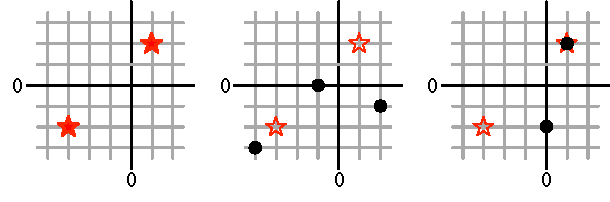
\includegraphics[width=.6\textwidth]{img/sample1.pdf}

Šiame pavyzdyje yra $k=2$ mineralų telkiniai koordinatėse $(1,2)$ ir $(-3,-2)$. Paveikslėlyje žymimi raudonomis žvaigždėmis.
Kaip pirmą grupę galėtumėte siųsti $d=3$ zondus į koordinates $(-4,-3)$, $(-1, 0)$ ir $(2,-1)$. Paveikslėlyje žymimi juodais taškais.
Ši grupė grąžintų $6$ atstumus: \[
  2, 4, 4, 4, 6, 10\,.
\]
Kaip kitą grupę, galėtumėte siųsti $d=2$ zondų į koordinates $(1,2)$ ir $(0,-2)$.
Ši grupė grąžintų $4$ atstumus: \[
  0, 3, 5, 8\,.
\]
